%This chapter addresses various design variants and challenges embedded with the proposed solution of moving a fine-grained scheduler to kernel space. 

In this chapter, we address the approach used for realizing IRS in kernel space. 
In the first section, we discuss a theoretical design. 
In the later sections, we address the potential challenges related to its implementation and the perceived prototypes.

\section{Theoretical Design}

The key component of this thesis is the scheduler. 
Scheduler handles the scheduling of various user level threads based on their memory access permissions. 
Memory access permissions are perceived by traces. 
The traces are realized simple graphs with nodes. 
Each node denotes a shared memory event for a thread which can be a read or a write event. 

\tikzstyle{custblock} = [rectangle, minimum width=3cm, minimum height=1cm, text centered, draw=black, fill=white!30]

\begin{figure}[h]
\centering
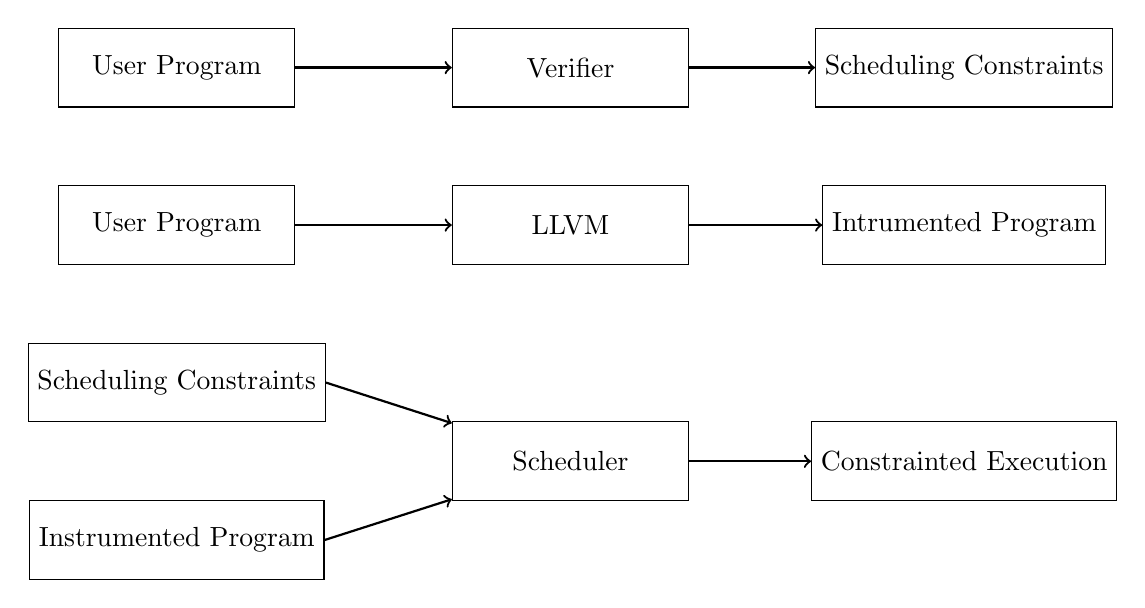
\begin{tikzpicture}[node distance=2cm]
%Custom blocks
\node (Us1) [custblock] {User Program};
\node (Us2) [custblock,below of=Us1] {User Program};
\node (ver) [custblock,right of=Us1,xshift =3cm] {Verifier};
\node (tr) [custblock,right of=ver,xshift =3cm] {Scheduling Constraints};
\node (llvm) [custblock,right of=Us2,xshift =3cm] {LLVM};
\node (ipgm) [custblock,right of=llvm,xshift =3cm] {Intrumented Program};
\node (Tr) [custblock,below of=Us2] {Scheduling Constraints};
\node (IPgm) [custblock,below of=Tr] {Instrumented Program};
\node (Sched) [custblock,right of=Tr,yshift=-1cm,xshift =3cm] {Scheduler};
\node (opgm) [custblock,right of=Sched,xshift =3cm] {Constrainted Execution};


%Arrows
\draw [->,thick] (Us1.east) -- (ver);
\draw [->,thick] (ver.east) -- (tr);
\draw [->,thick] (Us2.east) -- (llvm);
\draw [->,thick] (llvm.east) -- (ipgm);
\draw [->,thick] (Tr.east) -- (Sched);
\draw [->,thick] (IPgm.east) -- (Sched);
\draw [->,thick] (Sched.east) -- (opgm);
\end{tikzpicture}
\caption{IRS Design Overview}
\label{design_overview}
\end{figure}

The above figure depicts the design overview of the IRS. 
This thesis is based on the same design.  
Verifier is one of the main components of IRS. 
Verifier is not an automated software.
However, there are some changes in the representation of some components such as the trace/scheduling constraints which are discussed in the next section. 
\\
\noindent\begin{minipage}{.45\textwidth}
\begin{lstlisting}[mathescape=true,style=customc,caption=Uninstrumented User Program,frame=tlrb]{Name}
Shared Variable: x;
Thread j($j \in 1..N$): 
......
x=0;	//shared memory access
....
\end{lstlisting}
\label{uninstr_usr_pgm}
\end{minipage}\hfill
\begin{minipage}{.45\textwidth}
\begin{lstlisting}[mathescape=true,style=customc,caption=Instrumented User Program,frame=tlrb]{Name}
Shared Variable: x;
Thread j($j \in 1..N$): 
......
BeforeMA();
x=0;	//shared memory access
AfterMA();
....
\end{lstlisting}
\label{instr_usr_pgm}
\end{minipage}

LLVM is another component part of the IRS framework. 
It primarily annotates the user program for shared memory events as shown in listing 4.1 and 4.2. 

\subsection{Vector Clock}

Vector clock is an algorithmic design motivated from Lamport logical clocks~\citep{fidge1991logical}. 
It is used to detect causality violations and generating a partial ordering of events in a distributed system. 
A vector clock is an array of N logical clocks corresponding to N processes/threads. 
Vector clocks allow for the partial causal ordering of events.
The following definition holds:
\begin{itemize}
\item $VC(x)$ denotes the vector clock of event $x$, and $VC(x)_a$ denotes the component of that clock for process $a$. 
\item $VC(x) < VC(y) \iff \forall a[VC(x)_a \lneq VC(y)_a] \wedge \exists b[VC(x)_b < VC(y)_b]$
\item $x \to y$ indicates event $x$ happened before event $y$. It is defined as : if $x \to y$, then $VC(x) < VC(y)$
\end{itemize}

The design uses vector clock implementation for determining the number of memory events encountered by a given thread and use this information to block or unblock a given thread. 
The trace file generated as graph representations are manually converted into strings of vector clock representations for using in this thesis. 
The vector clock representation only include the threads which are constrainted. 
More details about the vector clock representation can be found in the appendix C.


\subsection{Design classes}

We have two different classes of approach used for this thesis. 
The two approaches can be classified as: design with proxy and design without proxy checking. 
Proxy checking referred above is the checking for memory  access permission for the thread based on the constraints set in the trace. 

\begin{lstlisting}[mathescape=true,style=customc,caption=Yield functionality and thread revival,frame=tlrb]{Name}
yield(threadid j) {
	if(memory_access_permission(j)==restricted) {
		block_thread(j);
	}
}
reviveotherthreads() {
	for Thread j($j \in 1..N$) except j is not the current thread:
		if(memory_access_permission(j)==allowed) {
			unblock_thread(j);
		}	
	}
}
\end{lstlisting}
\label{yield_func}
From figure~\ref{design_overview}, it is evident that we require scheduling constraints/traces and the instrumented program for executing with the scheduler. 
The IRS implementation which this thesis is based upon, uses an LLVM implementation for instrumenting the user program. 
When instrumenting the user program, LLVM inserts function calls to two methods namely $BeforeMA()$ and $AfterMA()$ which are inserted in places before and after every shared memory access in the program as shown in Listing~4.1 \& 4.2. 
The instrumented program is later, run with the scheduling constraints on the scheduler. 
The decision to block the thread is handled by the thread itself by invoking the yield functionality. 
A thread would block itself when it has no permission to access the shared memory. 
The decision making of the thread and the yield functionality are the only concepts discussed with the prototypes in this thesis. 

In this thesis, we propagate the decision making logic and yield functionality to kernel space as shown in Listing 4.3. 
However, in case of the second approach used in this thesis we have an additional proxy checking for memory permissions in user space. 
We expect these propogations to yield a good performance compared to the user space solutions. 

\noindent\begin{minipage}{.45\textwidth}
\begin{lstlisting}[mathescape=true,style=customc,caption=First Approach,frame=tlrb]{Name}
Thread j($j \in 1..N$): 
//on activating a BeforeMA call
BeforeMA() {
	yield(j);
}
AfterMA() {
	reviveotherthreads();
}
\end{lstlisting}
\label{first_approach}
\end{minipage}\hfill
\begin{minipage}{.45\textwidth}
\begin{lstlisting}[mathescape=true,style=customc,caption=Second Approach,frame=tlrb]{Name}
Thread j($j \in 1..N$): 
//on activating a BeforeMA call
BeforeMA() {
	if(memory_access_permission(j)==restricted) {
		yield(j);
	}
}
AfterMA() {
	reviveotherthreads();
}
\end{lstlisting}
\label{second_approach}
\end{minipage}


\subsubsection{First Approach}

This approach has no proxy checking in the user space. 
When there is an occurence of a shared memory event, this approach communicates to kernel space from the $BeforeMA()$ and $AfterMA()$ callback functions. 
These functions aid the logic of implementing yield functionality in the thread and also in reviving other threads. 
The pseudo implementation of this approach is depicted in listing 4.4.
There are four design prototypes using this approach. 
Details related to these prototypes are discussed further in this section.

\subsubsection{Second Approach}

This approach has a proxy checking in the user space. 
When there is an occurrence of a shared memory event, this approach initially checks for memory access permission and based on the outcome of the check, it communicates to the kernel space. 
$BeforeMA()$ and $AfterMA()$ functions are used in the same way as in first approach. 
However, with the only difference of having a proxy check for memory access permission inside the $BeforeMA()$. 
The pseudo implementation of this approach is depicted in listing 4.5.
There are two design prototypes using this approach. More details about these prototypes are discussed further in this section.
With the proxy checking in place, this design is expected to provide good performance when the following condition occurs: $num\_memory\_constraints << total\_memory\_events$. 
This approach reduces the number of unnecessary yield calls made to kernel space which reduces drastic overhead generated by communication and waiting in kernel space.



\section{Design Challenges}

\section*{Note}
In the progression of this document, we would be using certain acronyms to indicate certain meanings. 
Some of them are:
\begin{itemize}
\item \textbf{UTID} - User defined thread ID which is relative inside the user program. 
\item \textbf{RTID} - Real Thread ID which is assigned within the proc file system for any thread created within the user land. 
\item \textbf{TaskID} - All threads are internally realized as tasks in kernel space and are allocated with an identifier which is task ID.
\item \textbf{API} -Application Programming Interface.
\end{itemize}

\subsection{Mapping UTID to Task Object}

UTID  is passed to kernel space via a custom proc file and invoking scheduler API - $get\_current\_task()$. 
This function returns a task struct object. 
In kernel space, we can have a mapping of UTID to the obtained task struct object. 
User defined thread ID (UTID) is required to be communicated to the scheduler. 
And the mapping of task struct to UTID needs to be realized, in order for the scheduling to be done right. 
The custom registration proc file communicates the UTID to the kernel space. 
The user defined thread writes the UTID in the above proc file, which would trigger a callback to the write function in the kernel space module. 
Threads will be created based on the user's choice. 
On thread creation, the threads would invoke the registration module individually. 
This method would require a definition of synchronization block inside the kernel space since, multiple write function calls are invoked. 
Multiple threads are accessing the registration module. 
The synchronization is also required between the scheduler module and registration module.


\subsection{Data Structure for mapping UTID to Task Object}

The mapping of UTID - task object is realized, when the registration of a UTID to the scheduler is done. 
In the registration, the user thread is required to pass the UTID. 
The task object is obtained by invoking $get\_current\_task()$ function during registration call. 
The data structure is created to store the mapping of UTID to task object. 
An item in the data structure is created whenever a registration of UTID takes place. 
An item is otherwise accessed during the invocation of $context\_switch()$ function. 
In a user space environment, there are solutions such as dictionary mapper or even hash table designs. 
Since the mapping is coherent in the kernel space, possible design choices include - linked list, arrays. 
There is a complexity associated in accessing a node in the linked list, which is O(n).

\subsection{Communication between user thread and kernel space scheduler during context switch} 

With the transition of scheduler to kernel space, there is a need of having a communication design to interact between the user program and kernel space scheduler. 
The communication can be dealt in many ways\cite{commkernelanduser}. 
Some of them are:

\begin{itemize}
\item ProcFS - Virtual file system for handling process and thread information base. Useful for small and short communications. 
\item Netlink - Special IPC scheme between kernel space and user space which uses sockets. 
\item System call - Functional implementation mainly meant to communicate some data or perform a specific service in kernel space. 
\item CharacterDevice - Special buffering interface provided for communicating with character device driver setups.
\item Mmap - Fastest way of copying data between kernel space and user space without explicit copying. Useful for large transactions of data.
\item Signals - Unidirectional communication. Communicated from kernel space to user space. 
\item Upcall - Execute a certain function defined in the user space from kernel space.
\item IOCTL - Used primarily for input and output operations in between user space and kernel space. It is an extension of character device implementation. It uses simple read and write system calls for communication purposes. It can be realized as an alternative for system call.

\end{itemize}


Assessing the requirements for the implementation, IOCTL seems to be a perfect fit for all the interactions required for a scheduler module. 
System call implementation requires the building of the entire kernel source tree and they are very difficult to debug and develop. 
IOCTL provides the possibility for a plug and play design.

\subsection{Mapping the trace object to kernel space}

The proposed design uses vector clocks as an outline for trace implementation. 
The traces generated as graphs are mapped to kernel space a struct object. 
Graphs are realized as graphviz files. 
Parsing of graph is required in order to be mapped to the kernel space. 
The parsed graph is passed to the kernel space as a long string via a custom proc file. 
Currently, there is no automated method existent in this thesis to generate a graph string from a graphviz file. 
We generate the trace string manually and pass it as an input to the custom proc file when the user program starts.

\subsection{Trace verification inside user program vs kernel space scheduler}

On occurrence of a shared memory event, the respective callbacks (BeforeMA() \& AfterMA() - Before memory access and After memory access) from the user program would trigger a system call to the kernel module. 
Such a design would facilitate towards a non-preemptive scheduler. 
By overcoming the additional synchronization overhead existent in the user space design, we encounter the problem of invoking IOCTL calls  for accessing the kernel module. 
In a monolithic kernel architecture, most of the IOCTL calls are blocking synchronous calls to the kernel space. 
Having too many IOCTL calls would increase the scheduler overhead on the program execution. 
One solution is to make IOCTL calls when there is an actual need of a  context switch. 
The user space threads would assess the trace based on which the IOCTL calls for the kernel space scheduler would be made. 
We discuss about such a solution in two prototypes used in the implementation section.

Note - Non-preemptiveness indicated in this section and the rest of the document is in regard to the scheduler implemented in this thesis and not the OS Scheduler.

\subsection{Yield to scheduler vs Preemptive scheduler}

The current implementation uses a non-preemptive design for the scheduler. 
The design uses the verification of memory access event and performs yield to scheduler when the access to memory is not permitted. 
A preemptive design would reduce the communication between user space and kernel space during context switch but, would increase the same for every memory access events. 
With such an implementation, it would require the kernel space to be able to detect the memory access events of the global memory used by the user space threads. 
Considering the complexity of its implementation and lack of existing solutions such a design would be not feasible to implement. 


\subsection{Vector clock design for finding the event in the trace}

Before a shared memory access is made, the user thread triggers a callback - \emph{BeforeMA()} (in short before memory access). 
The callback internally triggers a yield to scheduler if the memory access is not permitted. 
The memory access permission is determined by checking the trace object. 
The timeline of the event is required to be addressed during the checking with the trace. 
The event timeline can be determined by having a vector clock design. 
The same vector design needs to be used inside the kernel space as well, for its trace verification function.


%----Implementation section------%

\section{Synchronization Designs}

We classify the designs in two classes for our convenience. 
The classification is based on the checking for memory permission in user space. 
The first class has no checking for memory permission in the user space and the second has a proxy checking in user space for memory permission. 

\begin{table}[h]
\begin{center}
 \begin{tabular}{|c c c|} 
 \hline
 & Shared Thread & Separate Thread\\ %[0.5ex] 
 \hline
Semaphore & Prototype 1 & Prototype 2\\
Scheduler APIs & Prototype 3 & Prototype 4\\
\hline
\end{tabular}
\end{center}
\caption{Prototypes without proxy checking}
\label{protos_without_proxy}
\end{table}

\begin{table}[h]
\begin{center}
 \begin{tabular}{|c c c|} 
 \hline
 & Shared Thread & Separate Thread\\ %[0.5ex] 
 \hline
Semaphore &  & Prototype 5\\
Scheduler APIs &  & Prototype 6\\
\hline
\end{tabular}
\end{center}
\caption{Prototypes with proxy checking}
\label{protos_with_proxy}
\end{table}


\subsection{Design with no checking in user space}

In the following designs, we address the use of check permission of memory access method entirely in Kernel space.

\subsubsection{Design with no additional scheduler thread} \label{no_check_no_add}

The design described in this section addresses the use of no additional scheduler thread. 


\subsubsection*{Trace Registration}

\begin{tikzpicture}[scale=0.7,transform shape]
 
  % Draw diagram elements
  % trace registration area
  \path \spacelayer {TRACEFILE}{Trace File}{Input to the scheduler};  
  \path (TRACEFILE.south)+(0.0,-2.0)\spacelayer {TRACEOBJ}{Trace Object}{Trace object is created and communicated to kernel space};  
  \path (TRACEOBJ.east)+(5.0,0.0) \spacelayer {TRACEPROCFS}{Trace Reg File}{Proc FS custom file for passing the trace object to kernel space};
  \path (TRACEPROCFS.east)+(4.5,0.0) \spacelayer {TRACESYSCALL}{SYSCALL\\ TRACE}{write() system call};  
  \path (TRACESYSCALL.south)+(0.0,-3.0) \spacelayer {TRACECALLBACK}{Trace Write Callback}{Callback function triggered inside LKM during write of trace object};
  
  % Draw arrows between elements

  %thread registration block
  \path [line] (TRACEFILE.south) -- node [left] {$trace$}
									 node [right] {$file$} (TRACEOBJ);
  \path [line] (TRACEOBJ.east) -- node [above] {$trace_reg()$} (TRACEPROCFS);

  \path [line] (TRACEPROCFS.east) -- node [above] {$write()$} (TRACESYSCALL);
  
  \path [linepart] (TRACESYSCALL.south) -- node [left] {$callback$}
                                 node [right]{$triggered$} (TRACECALLBACK);  
  
  %background generation block
  \background{TRACEFILE}{TRACEFILE}{TRACEOBJ}{TRACEOBJ}{User Space}
  \background{TRACESYSCALL}{TRACESYSCALL}{TRACECALLBACK}{TRACECALLBACK}{Kernel Space}

\end{tikzpicture}

The trace file is passed on as an input for the scheduler. 
In the above flow diagram, the trace file is read by the main user thread at the start of its execution. 
It parses the file, creates and passes the trace object to the kernel space as string via a custom file created in the proc file system. 

\subsubsection*{Thread Registration}

\begin{tikzpicture}[scale=0.7,transform shape] 
  
  % thread registration block area
  \path \spacelayer {THREADINIT}{Thread\\ Created}{thread\_init()};  
  \path (THREADINIT.south)+(0.0,-2.0)\spacelayer {USERTHREADREG}{Thread\\ Registration}{reg\_thread()};  
  \path (USERTHREADREG.east)+(5.0,0.0) \spacelayer {REGPROCFS}{Registration File}{Proc FS custom file for communication};
  \path (REGPROCFS.east)+(4.5,0.0) \spacelayer {REGSYSCALL}{SYSCALL\\ THREAD\\ REGISTRATION}{write() system call};
  \path (REGSYSCALL.south)+(0.0,-2.0) \spacelayer {REGCALLBACK}{Write Callback}{Callback function triggered inside LKM during write of thread ID};

  \background{THREADINIT}{THREADINIT}{USERTHREADREG}{USERTHREADREG}{User Space}
  \background{REGSYSCALL}{REGSYSCALL}{REGCALLBACK}{REGCALLBACK}{Kernel Space}
  
   %Draw arrows between elements
   %thread registration block
  \path [line] (THREADINIT.south) -- node [left] {$register$}
									 node [right] {$thread$} (USERTHREADREG);
  \path [line] (USERTHREADREG.east) -- node [above] {$reg_thread()$} (REGPROCFS);

  \path [line] (REGPROCFS.east) -- node [above] {$write()$} (REGSYSCALL);
  
  \path [linepart] (REGSYSCALL.south) -- node [left] {$callback$}
                                 node [right]{$triggered$} (REGCALLBACK);

\end{tikzpicture}

In the above picture, the registration block happens when a user thread is created. 
The registration happens via a custom proc file system. 




\subsubsection*{Memory Assessment}

Prior to any global memory access, the given design would invoke \emph{IOCTL} command with \emph{CTXT\_SWITCH} and thread id of the thread which addressed the memory event as its parameters. 


\begin{tikzpicture}[scale=0.7,transform shape]
 
 
  % memory assessment area
  
  \path \spacelayer {BEFOREMA}{Before M.A}{A callback is triggered before memory access is made to the global memory};
  \path (BEFOREMA.south)+(0.0,-2.0) \spacelayer {REQCTXTSWITCH}{Request \\ Context Switch}{ioctl(CTXT\_SWITCH, tid)};
  
  \path (REQCTXTSWITCH.south)+(0.0,-2.0) \spacelayer {MEMACCESS}{Memory\\ Access}{The Actual global Memory Access by the thread};

  \path (MEMACCESS.south)+(0.0,-2.0) \spacelayer {AFTERMA}{After M.A}{A callback is triggered after memory access is made to the global memory};
  \path (AFTERMA.south)+(0.0,-3.0) \spacelayer {USRSIGOTHERS}{Request \\ Signal Other Threads}{ioctl(SIG\_OTHERS, tid)};  
  
  
  \path (REQCTXTSWITCH.east)+(8.0,2.0) \spacelayer {CONTEXTSWITCH}{Context Switch call}{If memory access is restricted, signal\_other\_threads() and call down(thread\_sem[tid]) }; 
  \path (CONTEXTSWITCH.east)+(3.0,-5.0) \spacelayer {CHECKTRACE}{Check trace}{Checks if the execution in the input trace is valid or not.}; 
  \path (CONTEXTSWITCH.west)+(-2.0,-6.0) \spacelayer {THREADSEM}{THREAD\\ Semaphore}{Array of semaphores used by corresponding thread. Up and Down calls are made.}; 
 \path (CONTEXTSWITCH.south)+(0.0,-10.0) \spacelayer {SIGNALOTHERS}{Signal other\\ Threads}{Signals all the permitted threads to be resumed by calling up() on their respective semaphores. For verifying the permission internal call is made to checktrace}; 
 
  
  

  % Draw arrows between elements

 
 
  

  %memory assessment block
  \path [line] (BEFOREMA.south) -- node [left] {$req$} (REQCTXTSWITCH);
  \path [line] (AFTERMA.south) -- node [left] {$req$} (USRSIGOTHERS);

  \path [line] (REQCTXTSWITCH.east) -- node [midway,above,sloped] {$ioctl()$} (CONTEXTSWITCH);
  
  \path [line] (CONTEXTSWITCH.south) -- node [left] {} (CHECKTRACE);
  \path [line] (CONTEXTSWITCH.south) -- node [midway,above,sloped] {down(sem[tid])} (THREADSEM);
  \path [line] (CONTEXTSWITCH.south) -- node [left] {} (SIGNALOTHERS);
  \path [line] (CHECKTRACE.north) -- node [midway,above,sloped] {allowed\ or\ restricted} (CONTEXTSWITCH);  
   
  \path [line] (SIGNALOTHERS.north) -- node [left] {} (CHECKTRACE);   
  \path [line] (CHECKTRACE.south) -- node [midway,above,sloped] {allowed\ or\ restricted} (SIGNALOTHERS);
  \path [line] (SIGNALOTHERS.north) -- node [midway,above,sloped] {up(sem[tid])} (THREADSEM);
   
   \path [line] (USRSIGOTHERS.east) -- node [midway,above,sloped] {$ioctl()$} (SIGNALOTHERS);
  %\path [linepart] (CONTEXTSWITCH.west) -- node [above] {$thread$}
                                 %node [right]{$resume$} (THREADRESUME);

  %background generation block
 
  \background{BEFOREMA}{BEFOREMA}{USRSIGOTHERS}{USRSIGOTHERS}{User Space}
  \background{THREADSEM}{CONTEXTSWITCH}{CHECKTRACE}{SIGNALOTHERS}{Kernel Space}
  

\end{tikzpicture}


\newpage
\subsubsection*{Pseudo Implementation}
\begin{lstlisting}[title=Data Types Section used by user space and kernel space, style=customc]
enum IOCTL CMDS  { 
	GET_CURR_CLK = 1, 
  	CTXT_SWITCH = 2, 
  	SIGNAL_OTHER_THREADS = 3,
  	RESET_CLK = 4,
  	SET_MY_CLK = 5
}
\end{lstlisting}

\begin{lstlisting}[title=Check Permission for memory access, style=customc]
mem_access check_mem_acc_perm(vec_clk* curr_vec_clk, vec_clk* trace_inst, thread_id_t tid) {

   int i;
   if(trace_inst->clocks[tid-1] == curr_vec_clk->clocks[tid-1]) 
   {
     for i in range(0, THREAD_COUNT) 
     {
	if(i!=(tid-1)) 
	{
	 if(trace_inst->clocks[i] <= curr_vec_clk->clocks[i]) 
	 {
	 	continue;
	 }
	 else 
	 {
	 	return e_ma_restricted;
	 }
	}
     }
   }
   else if(trace_inst->clocks[tid-1] < curr_vec_clk->clocks[tid-1]) 
   {
   	return e_ma_restricted;
   }
   return e_ma_allowed;
}

\end{lstlisting}


\begin{lstlisting}[title=User Space Implementation, style=customc]
BeforeMA() {	
	ioctl(CTXT_SWITCH, thread_id);	
}

AfterMA() {	
	ioctl(SIGNAL_OTHER_THREADS, thread_id);
}

reset_clock() {
	ioctl(RESET_CLK);
}

//This method is defined by the thread library which is used by the user
thread_create_impl(thread t) {
	t ->thread_init(tid);
	t ->thread_exec(thread_function);
}

thread_function() {
	reg_thread();	//This method increments a threadcount variable in kernel space.
	....	
	Before_MA(); 	//function triggered before accessing the global memory
	Mem_Access();   //global memory access permitted for the thread
	AfterMA();		//function triggered after accessing the global memory		
	....
	thread_exit()
}

trace_reg() {	
	fd = open("/proc/trace_reg",O_RDWR);
	close(fd);	
}

main() {	
	trace_reg()
	thread t = thread_create(tid, thread_function); 
	//thread_create_impl() is called internally
	.....
	t.join();	
	return EXIT_SUCCESS;
}


\end{lstlisting}

\newpage
\begin{lstlisting}[title=Kernel Space - IOCTL, style=customc]
/* This method is triggered whenever ioctl commands are issued from the user space */
ioctl_access(IOCTL_CMDS cmd) {	
	switch(cmd) {
		case CTXT_SWITCH: 
			req_ctxt_switch(thread_id);//requests for context switch
			break;
		case SIGNAL_OTHER-THREADS:
			Increment_curr_clk(thread_id); //this will increment the current clk for the given thread id.
			signal_all_other_threads(thread_id);
			break;
		case GET_CURR_CLK:
			get_curr_clk();//returns the current vector clock.
			break;
		case RESET_CLK:
			reset_clk(); //reset the current vector clock to zero.
			break:		
		case SET_CURR_CLK:
			set_curr_clk(clk);//sets the current vector clock with the clk received.
	}
}

//Methods of interest with respect to the ioctl cmds
mem_access check_mem_access_with_trace(thread_id_t tid) {
	...
	//method internally calls check_mem_acc_perm() with current clock time and uses the first valid instance vector clock registered for a given thread in the trace array.
		
	//returns e_ma_allowed|e_ma_restricted based on the check_mem_acc_perm()
}

ctxt_switch_thread(thread_id_t tid) {	
	down(threads_sem[tid-1]); //perform semaphore down operation respective semaphore.
	/**if the value is already 0 when performing the down, the thread waits until the value is positive.*/
}

signal_all_other_threads(thread_id_t tid) {
	//critical section for wait queue
	up(threads_sem[i])$\forall$	
	//critical section ends.
}

req_ctxt_switch(thread_id_t tid) {
		if(check_mem_access_with_trace(tid) == e_ma_restricted) {

		signal_all_other_threads(tid);
		
		//critical section for waitqueue
		wait_queue[tid-1] = 1; //sets the thread inline for waiting
		//critical section ends.
		
		ctxt_switch_thread(tid);

	}
}

\end{lstlisting}

\subsubsection{Design with an additional scheduler thread}\label{sec_add_thread}

In this design, we create an additional scheduler thread primarily addressing the signaling mechanism pertained in the previous design. 
By having an additional scheduler thread, we move the entire signaling system to the scheduler thread.
Thus, reducing the execution overhead encountered in the user space thread for signaling other threads.

The major change from the previous design apart from additional thread is in the memory assessment block.

\subsubsection*{Memory assessment block}
\begin{tikzpicture}[scale=0.7,transform shape]
 
 
  % memory assessment area
  
  \path \spacelayer {BEFOREMA}{Before M.A}{A callback is triggered before memory access is made to the global memory};
  \path (BEFOREMA.south)+(0.0,-2.0) \spacelayer {REQCTXTSWITCH}{Request \\ Context Switch}{ioctl(CTXT\_SWITCH, tid)};
  
  \path (REQCTXTSWITCH.south)+(0.0,-2.0) \spacelayer {MEMACCESS}{Memory\\ Access}{The Actual global Memory Access by the thread};

  \path (MEMACCESS.south)+(0.0,-2.0) \spacelayer {AFTERMA}{After M.A}{A callback is triggered after memory access is made to the global memory};
  \path (AFTERMA.south)+(0.0,-3.0) \spacelayer {SETCLK}{Setting \\ Global Vector clock}{ioctl(SET\_CLK, tid)};  
  
  
  \path (REQCTXTSWITCH.east)+(9.0,2.0) \spacelayer {CONTEXTSWITCH}{Context Switch call}{If memory access is restricted, signal\_other\_threads() and call down(thread\_sem[tid]) }; 
  \path (CONTEXTSWITCH.east)+(3.0,-5.0) \spacelayer {CHECKTRACE}{Check trace}{Checks if the execution in the input trace is valid or not.}; 
  \path (CONTEXTSWITCH.west)+(-2.0,-6.0) \spacelayer {THREADSEM}{THREAD\\ Semaphore}{Array of semaphores used by corresponding thread. Up and Down calls are made.}; 
  \path (CONTEXTSWITCH.south)+(0.0,-10.0) \spacelayer {SIGNALOTHERS}{Signal other\\ Threads}{Signals all the permitted threads to be resumed by calling up() on their respective semaphores. For verifying the permission internal call is made to checktrace}; 
 \path (SIGNALOTHERS.west)+(-3.0,0.0) \spacelayer {SETVECCLK}{Set Vector\\ Clock}{Kernel adaptation of set vector clock method invoked on ioctl call.}; 
 \path (SIGNALOTHERS.east)+(+3.0,0.0) \spacelayer {ADDTHREAD}{Additional\\ Thread}{Additional thread invokes signalothers method for every x ms.};  
  

  % Draw arrows between elements

 
 
  

  %memory assessment block
  \path [line] (BEFOREMA.south) -- node [left] {$req$} (REQCTXTSWITCH);
  \path [line] (AFTERMA.south) -- node [left] {$req$} (SETCLK);

  \path [line] (REQCTXTSWITCH.east) -- node [midway,above,sloped] {$ioctl()$} (CONTEXTSWITCH);
  
  \path [line] (CONTEXTSWITCH.south) -- node [left] {} (CHECKTRACE);
  \path [line] (CONTEXTSWITCH.south) -- node [midway,above,sloped] {down(sem[tid])} (THREADSEM);
  \path [line] (CONTEXTSWITCH.south) -- node [left] {} (SIGNALOTHERS);
  \path [line] (CHECKTRACE.north) -- node [midway,above,sloped] {allowed\ or\ restricted} (CONTEXTSWITCH);  
   
  \path [line] (SIGNALOTHERS.north) -- node [left] {} (CHECKTRACE);   
  \path [line] (CHECKTRACE.south) -- node [midway,above,sloped] {allowed\ or\ restricted} (SIGNALOTHERS);
  \path [line] (SIGNALOTHERS.north) -- node [midway,above,sloped] {up(sem[tid])} (THREADSEM);
   
   \path [line] (SETCLK.east) -- node [midway,above,sloped] {$ioctl()$} (SETVECCLK);
  %\path [linepart] (CONTEXTSWITCH.west) -- node [above] {$thread$}
                                 %node [right]{$resume$} (THREADRESUME);
   \path [line] (ADDTHREAD.west) -- node [left] {} (SIGNALOTHERS);
  %background generation block
 
  \background{BEFOREMA}{BEFOREMA}{SETCLK}{SETCLK}{User Space}
  \background{SETVECCLK}{CONTEXTSWITCH}{CHECKTRACE}{SIGNALOTHERS}{Kernel Space}
  

\end{tikzpicture}
\newpage
\subsubsection*{Pseudo Implementation}

The major changes are in kernel space code. 
However, there are minor variations in the \emph{AfterMA()} in user space. 

\begin{lstlisting}[title=User Space Implementation, style=customc]
//Rest of the code remains the same

AfterMA() {	
	ioctl(SET_MY_CLK, thread_id);
}

//Rest of the code remains the same

\end{lstlisting}

\begin{lstlisting}[title=Kernel Space - General module definitions, style=customc]
//code remains the same

signal_permitted_threads() {
	//critical section for wait queue
	for i in(0,THREAD_COUNT) {
		if(wait_queue[i] == 1) {
			if(check_mem_access_with_trace(i+1) == e_ma_allowed) {
				/**Performs up operation on the respective thread semaphore.*/
				up(threads_sem[i]);
				wait_queue[i]=0;			
			}		
		}
	}	
	
	//critical section ends.
}

module_init() {
	//code remains the same
	
	kernel_thread tk = create_kernel_thread(signal_permitted_threads)
	tk->setTimerCallForEvery(x) //this method will make call to signal permitted threads for every x ms.
}

//code remains the same
\end{lstlisting}


\subsection{Design with checking in user space}

In the following designs, we address the use of check permission of memory access method both in User Space and Kernel space.

\subsubsection{Design with no additional scheduler thread}

Without an additional thread in kernel space, the design would require a signaling function inside \emph{AfterMA()}, similar to the one used in Design~\ref{no_check_no_add}. 
Triggering a signaling mechanism is an additional overhead on the thread calling the \emph{AfterMA()}. 
Therefore, such a design is not a wise choice when considering the performance metrics such as execution time.
 
\subsubsection{Design with an additional scheduler thread}

The scheduler implementation is similar to one defined in the section \ref{sec_add_thread}. 
Key difference is the additional checking for memory permissions in the user space. 

\subsubsection*{Memory assessment block}
\begin{tikzpicture}[scale=0.7,transform shape]
 
 
  % memory assessment area

  \path \spacelayer {BEFOREMA}{Before M.A}{A callback is triggered before memory access is made to the global memory. If memory access is restricted, req\_ctxt()};
  \path (BEFOREMA.south)+(-3.0,-2.5) \spacelayer {CHECKTRACEUSR}{Check trace}{Checks if the execution in the input trace is valid or not.};   
  
  \path (BEFOREMA.south)+(0.0,-6.0) \spacelayer {REQCTXTSWITCH}{Request \\ Context Switch}{ioctl(CTXT\_SWITCH, tid)};
  
  \path (REQCTXTSWITCH.south)+(-3.0,-2.0) \spacelayer {MEMACCESS}{Memory\\ Access}{The Actual global Memory Access by the thread};

  \path (MEMACCESS.south)+(3.0,-2.0) \spacelayer {AFTERMA}{After M.A}{A callback is triggered after memory access is made to the global memory};
  \path (AFTERMA.south)+(0.0,-3.0) \spacelayer {SETCLK}{Setting \\ Global Vector clock}{ioctl(SET\_CLK, tid)};  
  
  
  \path (REQCTXTSWITCH.east)+(9.0,2.0) \spacelayer {CONTEXTSWITCH}{Context Switch call}{If memory access is restricted, signal\_other\_threads() and call down(thread\_sem[tid]) }; 
  \path (CONTEXTSWITCH.east)+(3.0,-5.0) \spacelayer {CHECKTRACE}{Check trace}{Checks if the execution in the input trace is valid or not.}; 
  \path (CONTEXTSWITCH.west)+(-2.0,-6.0) \spacelayer {THREADSEM}{THREAD\\ Semaphore}{Array of semaphores used by corresponding thread. Up and Down calls are made.}; 
  \path (CONTEXTSWITCH.south)+(0.0,-10.0) \spacelayer {SIGNALOTHERS}{Signal other\\ Threads}{Signals all the permitted threads to be resumed by calling up() on their respective semaphores. For verifying the permission internal call is made to checktrace}; 
 \path (SIGNALOTHERS.west)+(-3.0,0.0) \spacelayer {SETVECCLK}{Set Vector\\ Clock}{Kernel adaptation of set vector clock method invoked on ioctl call.}; 
 \path (SIGNALOTHERS.east)+(+3.0,0.0) \spacelayer {ADDTHREAD}{Additional\\ Thread}{Additional thread invokes signalothers method for every x ms.};  
  

  % Draw arrows between elements

 
 
  

  %memory assessment block
  \path [line] (BEFOREMA.south) -- node [left] {} (CHECKTRACEUSR);
  \path [line] (CHECKTRACEUSR.south) -- node  [midway,right] {$restricted$} (REQCTXTSWITCH);
  \path [line] (CHECKTRACEUSR.south) -- node  [left] {$allowed$} (MEMACCESS);
  \path [line] (AFTERMA.south) -- node [left] {$req$} (SETCLK);

  \path [line] (REQCTXTSWITCH.east) -- node [midway,above,sloped] {$ioctl()$} (CONTEXTSWITCH);
  
  \path [line] (CONTEXTSWITCH.south) -- node [left] {} (CHECKTRACE);
  \path [line] (CONTEXTSWITCH.south) -- node [midway,above,sloped] {down(sem[tid])} (THREADSEM);
  \path [line] (CONTEXTSWITCH.south) -- node [left] {} (SIGNALOTHERS);
  \path [line] (CHECKTRACE.north) -- node [midway,above,sloped] {allowed\ or\ restricted} (CONTEXTSWITCH);  
   
  \path [line] (SIGNALOTHERS.north) -- node [left] {} (CHECKTRACE);   
  \path [line] (CHECKTRACE.south) -- node [midway,above,sloped] {allowed\ or\ restricted} (SIGNALOTHERS);
  \path [line] (SIGNALOTHERS.north) -- node [midway,above,sloped] {up(sem[tid])} (THREADSEM);
   
   \path [line] (SETCLK.east) -- node [midway,above,sloped] {$ioctl()$} (SETVECCLK);
  %\path [linepart] (CONTEXTSWITCH.west) -- node [above] {$thread$}
                                 %node [right]{$resume$} (THREADRESUME);
   \path [line] (ADDTHREAD.west) -- node [left] {} (SIGNALOTHERS);
  %background generation block
 
  \background{CHECKTRACEUSR}{BEFOREMA}{SETCLK}{SETCLK}{User Space}
  \background{SETVECCLK}{CONTEXTSWITCH}{CHECKTRACE}{SIGNALOTHERS}{Kernel Space}
  

\end{tikzpicture}
\subsubsection*{Pseudo Implementation}

The major changes are in user space code. 


\begin{lstlisting}[title=User Space Implementation, style=customc]
//Rest of the code remains the same


mem_access ma_status[THREAD_COUNT];
vec_clk curr_clk_time;

initialize_vec_clock() {

    for i in range(0, THREAD_COUNT)
    {
        curr_clk_time.clocks[i] = 0;
    }
}

BeforeMA() {

	ma_status[thread_id-1] = check_mem_access_with_trace(thread_id);
	if(ma_status[id-1] == e_ma_restricted) {
		ioctl(CTXT_SWITCH, thread_id);	
	}
	  
}

AfterMA() {	
	ioctl(SET_MY_CLK, thread_id);
	curr_clk_time.clocks[thread_id-1]++;
}

//Rest of the code remains the same

\end{lstlisting}

\subsection{Variant in blocking implementation}

In the previous designs, the blocking was done using semaphores. 
In the variant design, we use the combination of \emph{schedule()} and \emph{wake\_up\_process()} functions provided by the Linux scheduler APIs. 
The kernel level tasks associated for the provided user level threads are moved from running queue to wait queue by initially setting the task status as \emph{TASK\_INTERRUPTIBLE} and yielding the processor by invoking \emph{schedule()}. 
The task added in wait queue is later resumed, when \emph{wake\_up\_process(sleeping\_task)} is invoked by another task. 
On calling the \emph{wake\_up\_process(sleeping\_task)}, the task status for \emph{sleeping\_task} is set as \emph{TASK\_RUNNING}. 
It would be pushed to run queue and executed in future by the operating system scheduler on the basis of scheduler class and priority of tasks in run queue. 
 
 
\subsubsection*{Variant Pseudo Code for Design \ref{no_check_no_add}}


\begin{lstlisting}[title=Kernel Space - IOCTL, style=customc]
//code remains the same

ctxt_switch_thread(thread_id_t tid) {	
	//critical section for wait queue
	wait_queue[tid-1].is_waiting = 1;
	wait_queue[tid-1].my_task = current;
	set_current_state(TASK_INTERRUPTIBLE);
	//critical section ends
	schedule();
}

signal_all_other_threads(thread_id_t tid) {
	//critical section for wait queue
	for i in(0,THREAD_COUNT) {
		if(i!=(tid-1)&&(wait_queue[i].is_waiting==1)) {
			if(check_mem_access_with_trace(i+1) == e_ma_allowed) {
				wait_queue[i].is_waiting = 0;
				wake_up_process(wait_queue[i].my_task);				
			}		
		}
	}	
	
	//critical section ends.
}


\end{lstlisting}

\subsubsection*{Variant Pseudo Code for Design \ref{sec_add_thread}}

\begin{lstlisting}[title=Kernel Space - General module definitions, style=customc]
//code remains the same

signal_permitted_threads() {
	//critical section for wait queue
	for i in(0,THREAD_COUNT) {
		if(wait_queue[i].is_waiting==1) {
			if(check_mem_access_with_trace(i+1) == e_ma_allowed) {
				/**Performs up operation on the respective thread semaphore.*/
				wait_queue[i].is_waiting = 0;
				wake_up_process(wait_queue[i].my_task);	
			}		
		}
	}	
	
	//critical section ends.
}

//code remains the same
\end{lstlisting}
